Figure \ref{arduino_wiring_hmc.png} provides a wiring diagram for connectivity of a HMC6343 to an Arduino Uno R3, with the pinout values provided by table \ref{HMC6343wiringtable}. Figure \ref{arduino_joystick_for_second_life_1.jpg} shows the assembled unit.

\begin{figure}[h]
\centering
  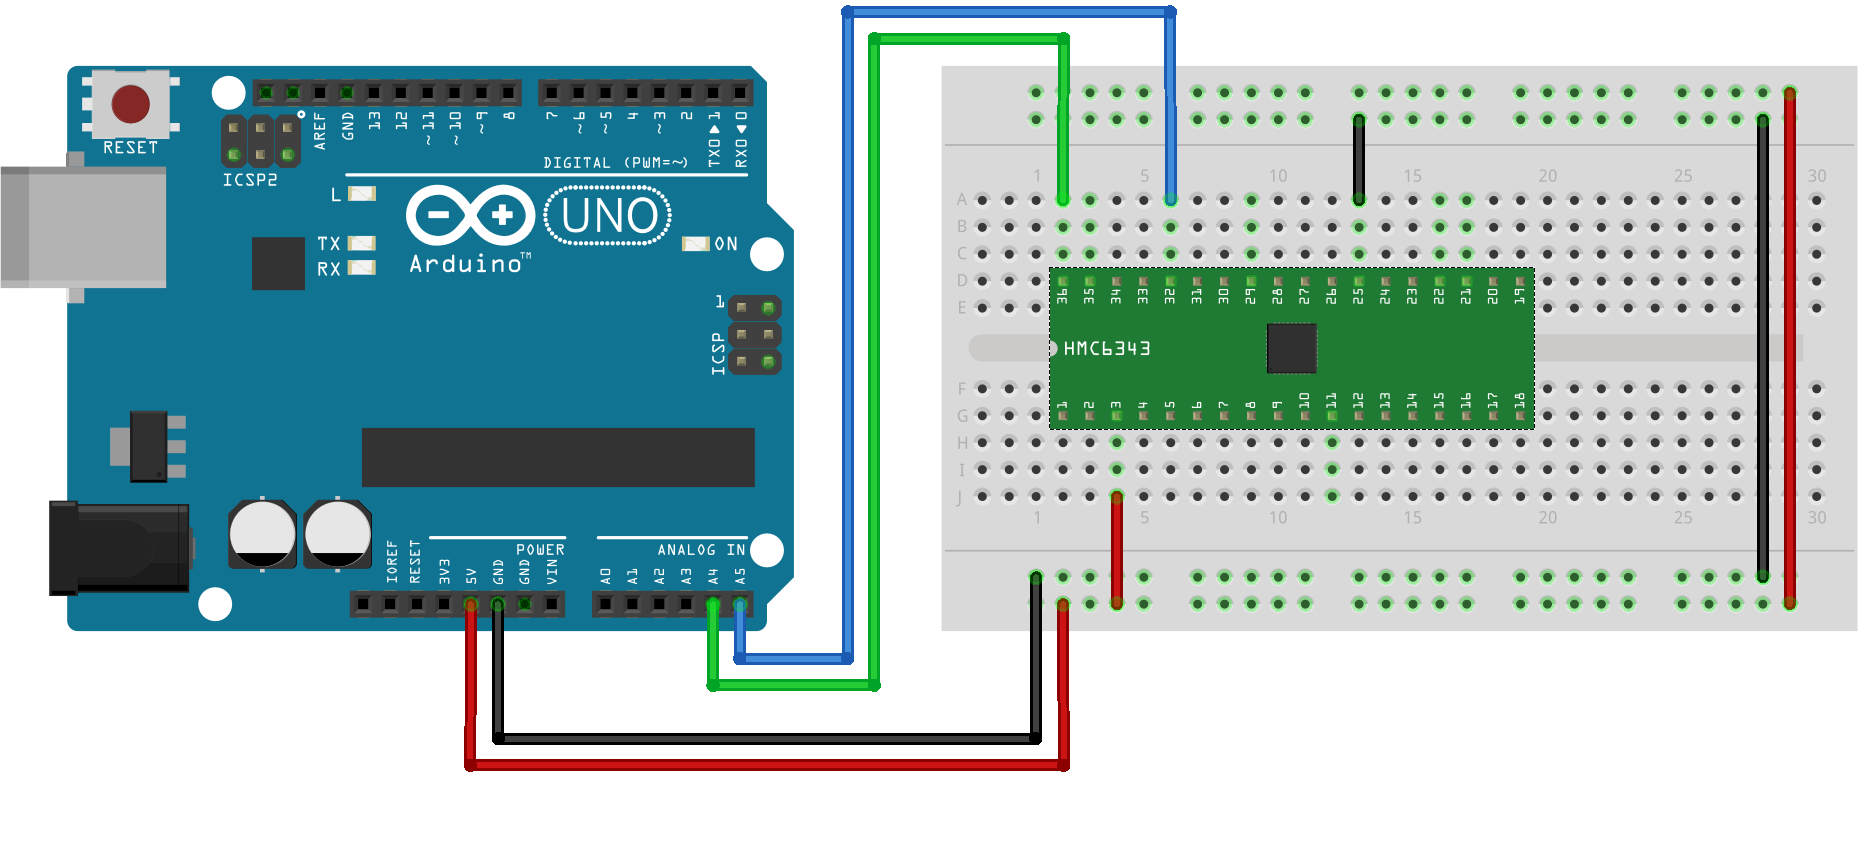
\includegraphics[width=\linewidth]{arduino_wiring_hmc.png}
  \caption{Wiring diagram for Arduino with HMC6343.}
  \label{arduino_wiring_hmc.png}
\end{figure}

%=====================

\begin{table}
%\begin{center}
\begin{minipage}[c]{.45\linewidth}
\begin{center}
\begin{tabularx}{\textwidth}{c *{2}{>{\centering\arraybackslash}X}}
\toprule
\textbf{HMC6343 pin} & \textbf{Arduino Uno R3 pin} \\
\midrule
VCC & 5V\HMCvccFootnote{} \\

GND & GND \\

SDA & A4\itwocFootnote{} \\

SCL & A5 \\
\bottomrule
\end{tabularx}
\caption{Pin designation for figure \ref{arduino_wiring_hmc.png}.}
\label{HMC6343wiringtable}
\end{center}
\end{minipage}
%
\begin{minipage}[c]{.02\linewidth}
\hfill%
\end{minipage}
%
\begin{minipage}[c]{.45\linewidth}
\begin{center}
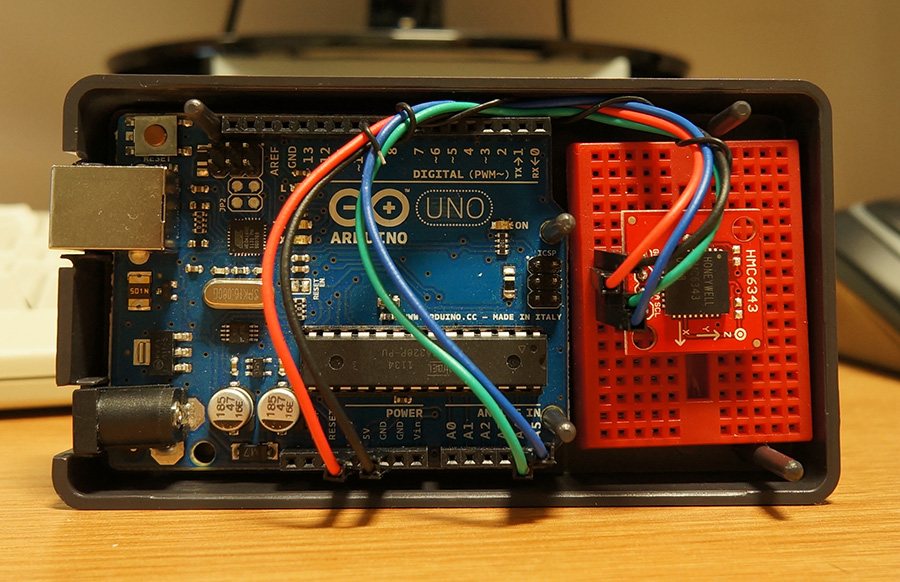
\includegraphics[width=\linewidth]{arduino_joystick_for_second_life_1.jpg}
\captionof{figure}{Assembled Arduino Uno R3 and HMC6343 package.}
\label{arduino_joystick_for_second_life_1.jpg}
\end{center}
\end{minipage}
%\end{center}
\end{table}

%=====================

\pagebreak

Figure \ref{arduino_wiring_hmc_ublox.png} provides a wiring diagram for connectivity of a u-blox MAX-6 to an Arduino Uno R3, along with the HMC6343 from section \ref{OrientationControl}, with the pinout values provided by tables \ref{HMC6343_MAX6_wiringtable_HMC6343} and \ref{HMC6343_MAX6_wiringtable_MAX6}. The LED and 220$\Omega$ resistor on digital pin 12 is used for diagnostic output. The wiring shown here is for a MAX-6 breakout without I$^{2}$C connectivity, instead using Arduino's SoftwareSerial\softwareserialFootnote{} library. Figure \ref{arduino_hmc6343_u-blox_MAX-6.jpg} shows the assembled unit, comprising an Arduino Uno R3, prototyping shield, HMC6343 and MAX-6, while figure \ref{pangolin_tablet_back.jpg} shows this package attached to the back of the WindPad with the single required USB cable connecting the two.

\begin{figure}[h]
\centering
  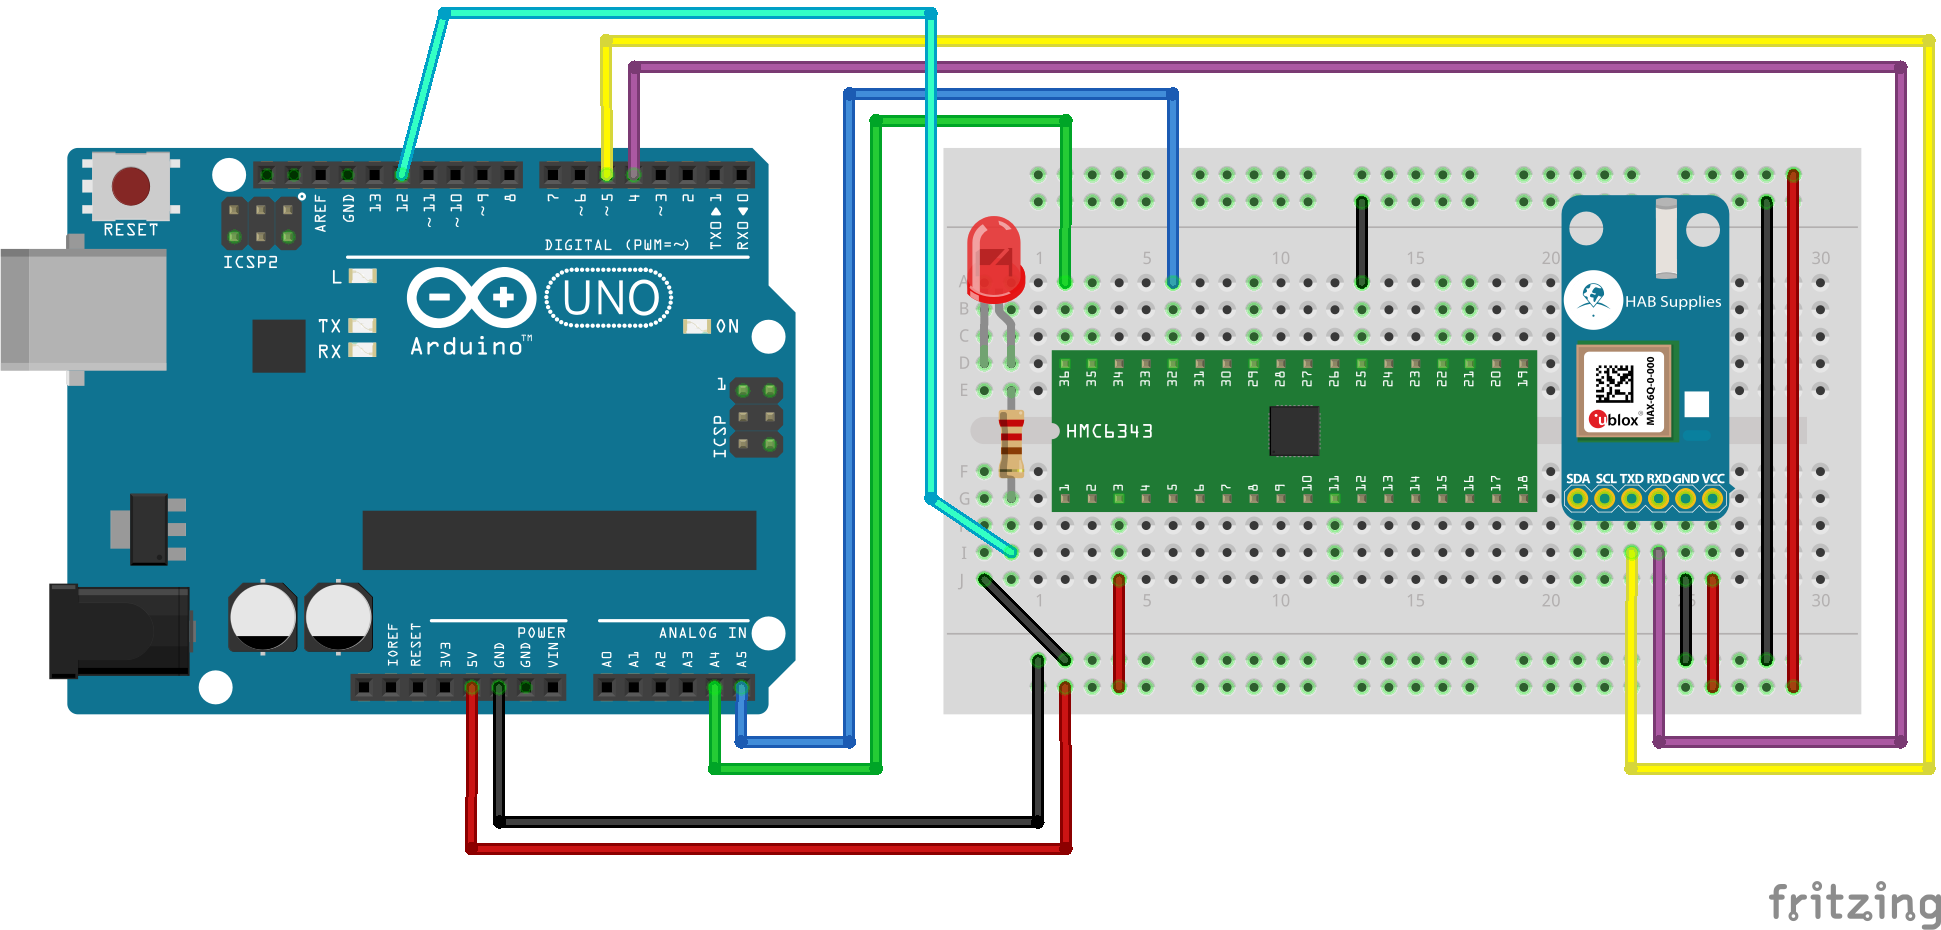
\includegraphics[width=\linewidth]{arduino_wiring_hmc_ublox.png}
  \caption{Wiring diagram for Arduino with HMC6343 and u-blox MAX-6.}
  \label{arduino_wiring_hmc_ublox.png}
\end{figure}

\begin{table}
\begin{center}
\begin{minipage}[t]{.45\linewidth}
\begin{center}
\begin{tabularx}{\textwidth}{c *{2}{>{\centering\arraybackslash}X}}
\toprule
\textbf{HMC6343 pin} & \textbf{Arduino Uno R3 pin} \\
\midrule
VCC & 5V\HMCvccFootnote{} \\

GND & GND \\

SDA & A4\itwocFootnote{} \\

SCL & A5 \\
\bottomrule
\end{tabularx}
\caption{Pin designation for figure \ref{arduino_wiring_hmc_ublox.png} (HMC6343).}
\label{HMC6343_MAX6_wiringtable_HMC6343}
\end{center}
\end{minipage}
%
\begin{minipage}[t]{.02\linewidth}
\hfill%
\end{minipage}
%
\begin{minipage}[t]{.45\linewidth}
\begin{center}
\begin{tabularx}{\textwidth}{c *{2}{>{\centering\arraybackslash}X}}
\toprule
\textbf{MAX-6 pin} & \textbf{Arduino Uno R3 pin} \\
\midrule
VCC & 5V\MAXvccFootnote{} \\

GND & GND \\

RXD & D4 \MAXserialFootnote{}\\

TXD & D5 \\
\bottomrule
\end{tabularx}
\caption{Pin designation for figure \ref{arduino_wiring_hmc_ublox.png} (MAX-6).}
\label{HMC6343_MAX6_wiringtable_MAX6}
\end{center}
\end{minipage}
\end{center}
\end{table}

\TwoFig{arduino_hmc6343_u-blox_MAX-6.jpg} {Assembled Arduino/sensor package used by VTW.} {arduino_hmc6343_u-blox_MAX-6.jpg}
       {pangolin_tablet_back.jpg} {Arduino/sensor package attached to tablet used by VTW.} {pangolin_tablet_back.jpg}

%=====================

The MAX-6 was configured as follows:

\begin{enumerate}
	\item Dynamic Platform Model set to Pedestrian.
	\item SBAS via EGNOS enabled.
	\item GPGLL/GPGSA/GPGSV/GPVTG messages disabled.
	\item GPRMC/GPGGA messages enabled.
\end{enumerate}

\begin{figure}[h]
\begin{lstlisting}[language=C, numbers=left, numberstyle=\small, stepnumber=1, frame=single, breaklines=true, backgroundcolor=\color{codebackground}, showstringspaces=false]
uint8_t CFG_NAV5[] = {0xB5, 0x62, 0x06, 0x24, 0x24, 0x00, 0xFF, 0xFF,
                      0x03, 0x03, 0x00, 0x00, 0x00, 0x00, 0x10, 0x27,
                      0x00, 0x00, 0x05, 0x00, 0xFA, 0x00, 0xFA, 0x00,
                      0x64, 0x00, 0x2C, 0x01, 0x32, 0x3C, 0x00, 0x00,
                      0x00, 0x00, 0x00, 0x00, 0x00, 0x00, 0x00, 0x00,
                      0x00, 0x00, 0x00, 0x00};
calculateUBXChecksum(CFG_NAV5, (sizeof(CFG_NAV5)/sizeof(uint8_t)));

while (!success)
{
  sendUBX(CFG_NAV5, (sizeof(CFG_NAV5)/sizeof(uint8_t)));
  success = getUBX_ACK(CFG_NAV5);
}
success = 0;
\end{lstlisting}
\caption{Setting MAX-6 Dynamic Platform Model to Pedestrian in an Arduino sketch.}
\label{arduinoMAX6hex}
\end{figure}

These hex arrays can be generated by hand from the UBX protocol specification\maxProtocolFootnote{}, or by connecting the MAX-6 directly to a host computer (such as by using an Arduino as a Universal Asynchronous Receiver/Transmitter (UART) by connecting the MAX-6 to digital pins 0 and 1) and using the u-blox u-center\footnote{\url{https://u-blox.com/en/evaluation-tools-a-software/u-center/u-center.html}} software, copying the resultant config as hex messages from the relevant console window.